\section{Portal by Example}
\label{sec:example}

In this section we present \ql, a declarative query language for
evolving graphs. \ql uses SQL-like syntax, and has the form
\insql{TSelect} \ldots \insql{From} \ldots \insql{TWhere} \ldots
\insql{TGroup}.  We prefix temporal keywords with \insql{T}, to make
the distinction between \ql and SQL operations explicit.  We will use
\tgs \insql{T1} and \insql{T2} of Figures~\ref{fig:tg}
and~\ref{fig:tg_t2}, with structural schema V(\underline{vid}:int,
name:str, salary:int); E(\underline{vid1}:int, \underline{vid2}:int,
cnt:int), in our examples.

\subsection{Portal Basics}
\label{sec:example:basics}

{\bf Temporal selection.}  Consider query $Q1$ below.  

\begin{figure}
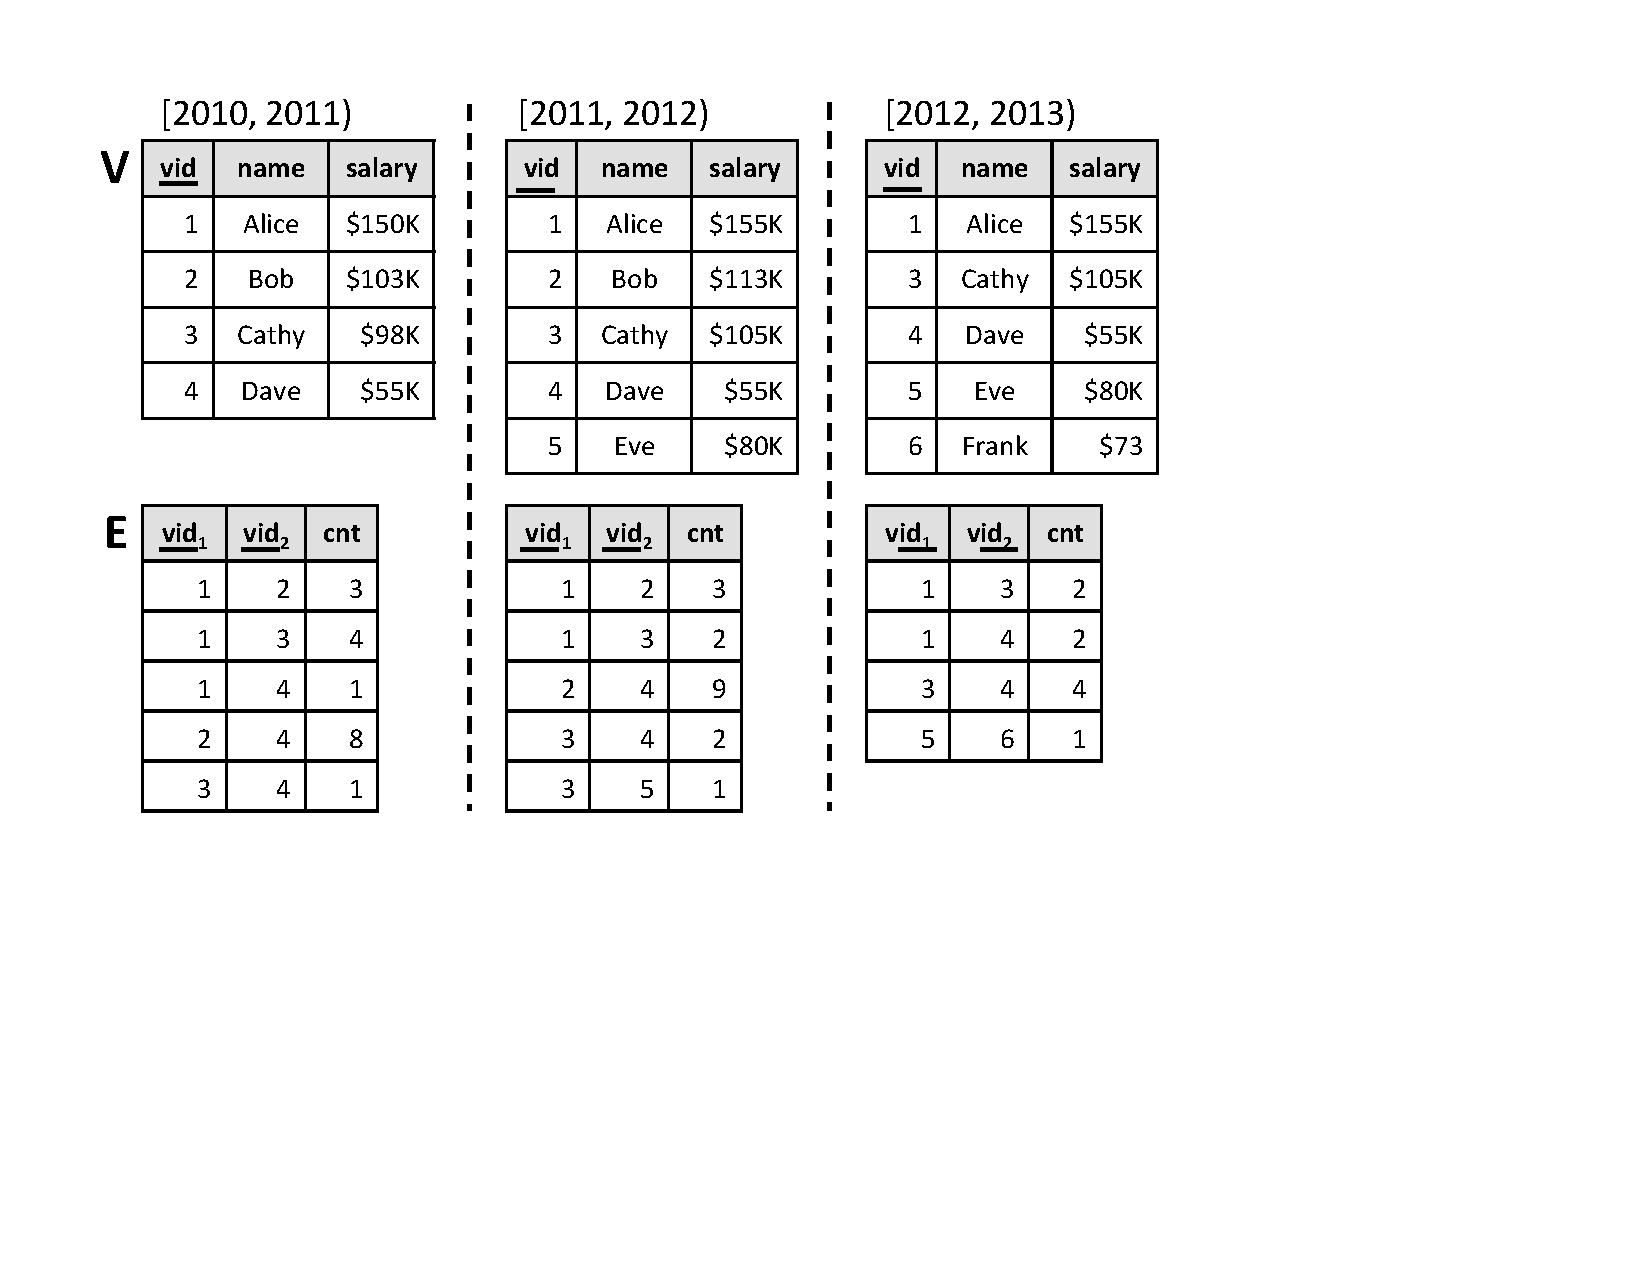
\includegraphics[width=3.5in]{figs/3VE.pdf}
\caption{Vertices and edges of 3 snapshots of \insql{T1}.}
\label{fig:3ve}
\end{figure}

\begin{small}
\begin{verbatim}
Q1: TSelect  V; E
    From     T1
    TWhere   Start >= 2010 And End <= 2014
\end{verbatim}
\end{small}

$Q1$ performs temporal selection --- its result is a \tg that contains
a consecutive subset of the snapshots of \insql{T1} that fall within
the interval specified by the \insql{TWhere} clause, namely, $[2010,
  2011)$ through $[2013, 2014)$.  The result of $Q1$ has the same
    structural schema as \insql{T1}. The \insql{Start} or the
    \insql{End} portions of the \insql{TWhere} clause may be omitted.

More generally, the \insql{TWhere} clause supports a variety of
predicates based on which it is determined, for each snapshot in a
\tg, whether that snapshot is to be retained or discarded.  For
example, \insql{TWhere month(Start) like '\%r\%'} will retain all
snapshots that start during a month in which it is safe to eat oysters
(these are months with the letter 'r' in their name), while
\insql{TWhere year(End) \% 4 = 0} will retain snapshots that end in a
leap year, and discard all others.  However, recall from
Definition~\ref{def:tseq} that a temporal sequence, which constitutes
the temporal schema of a \tg, cannot have any gaps.  We enforce this
by never discarding a time interval in the middle of a sequence, but
rather replacing its snapshot with an empty graph $G(V=\emptyset;
E=\emptyset)$.

\eat{\insql{Start} $t_1$ \insql{End} $t_2$ specifies a closed-open
  period $[t_1, t_2)$.  Its time unit must match, or be coarser than,
    the time unit of \insql{T1}.  If $t_1 < P.start$, we rewrite the
    query, setting $t_1 = P.start$.  Similarly, if $t_2 > P.end$, we
    rewrite the query, setting $t_2 = P.end$.  If $t_1$ does not fall
    on an interval boundary in the input \tg, we rewrite the query,
    setting $t_1$ to the {\em beginning} of the interval in which it
    falls.  If $t_2$ does not fall on the interval boundary, we rewrite
    the query, setting $t_2$ to the {\em end} of the interval in which}

{\bf Specifying structural schema of the result.  Snapshot analytics.}
Next, consider query $Q2$ below.

\begin{small}
\begin{verbatim}
Q2: TSelect  V [vid, pagerank() as pr]; 
             E [vid1, vid2, cnt * 0.001 as score]
    From     T1
\end{verbatim}
\end{small}

This query illustrates how the \insql{TSelect} clause can be used to
specify the structural schema of the result, which in this case is
V(\underline{vid}:int, pr:float); E(\underline{vid1}:int,
\underline{vid2}:int, score:float).  We may use the \insql{TSelect}
clause to project out non-key columns of \insql{V} and \insql{E}, or
to add columns with computed values.  Data types of computed
attributes \insql{pr} and \insql{score} are determined by the return
type of the expressions that compute them.  Note that key columns of
\insql{V} and \insql{E} must be present in the result.

The value of the attribute \insql{pr} in $Q2$ is computed using a
snapshot analytic function \insql{pagerank()}.  \ql supports a variety
of snapshot analytics --- functions whose values are computed
w.r.t. each snapshot of a \tg --- including degree, shortest paths,
and connected components.  We provide an API that allows developers to
implement custom analytics that can either be computed locally at a
vertex, like degree, or be expressed in the popular Pregel
API~\cite{DBLP:conf/sigmod/MalewiczABDHLC10}.

\subsection{Temporal Aggregation and Join}
\label{sec:example:groupjoin}

{\bf Temporal aggregation} is illustrated by query $Q3$, which, when
executed with \insql{T1} from Figure~\ref{fig:tg} as input, computes
the \tg in Figure~\ref{fig:q3}.

\begin{small}
\begin{verbatim}
Q3: TSelect   Any V ; Any E 
    From      T1
    TGroup    by 2 years
\end{verbatim}
\end{small}

Temporal aggregation is a two-step operation.  First, temporal schema
of the output is computed according to Definition~\ref{def:tgroup}.
Then structural aggregation of Definition~\ref{def:sgroup} is used
over snapshots in the same temporal group.  Note the use of \insql{Any
  V} and \insql{Any E} in the \insql{TSelect} clause of $Q3$,
specifying that $\gamma^{V}$ and $\gamma^{E}$ operate over unions of
vertices and edges.  For an example consider snapshot $[2010, 2012)$
  in Figure~\ref{fig:q3}, which is computed from snapshots $[2010,
    2011)$ and $[2011, 2012)$ of \insql{T1} in Figure~\ref{fig:tg}.

\eat{
Recall that temporal aggregation in \ql is semantic, in that we can
aggregate an input \tg that has day as its unit into a \tg with month
as its time unit, by simply specifying \insql{TGroup by 1 month}, and
without having to worry about how many days there are in a particular
month.}

We may use \insql{TGroup by Size} to specify that all snapshots of the
input \tg be aggregated into a 1-snapshot \tg.  This notation will be
useful when we discuss trend analytics later in this section.

\begin{figure}
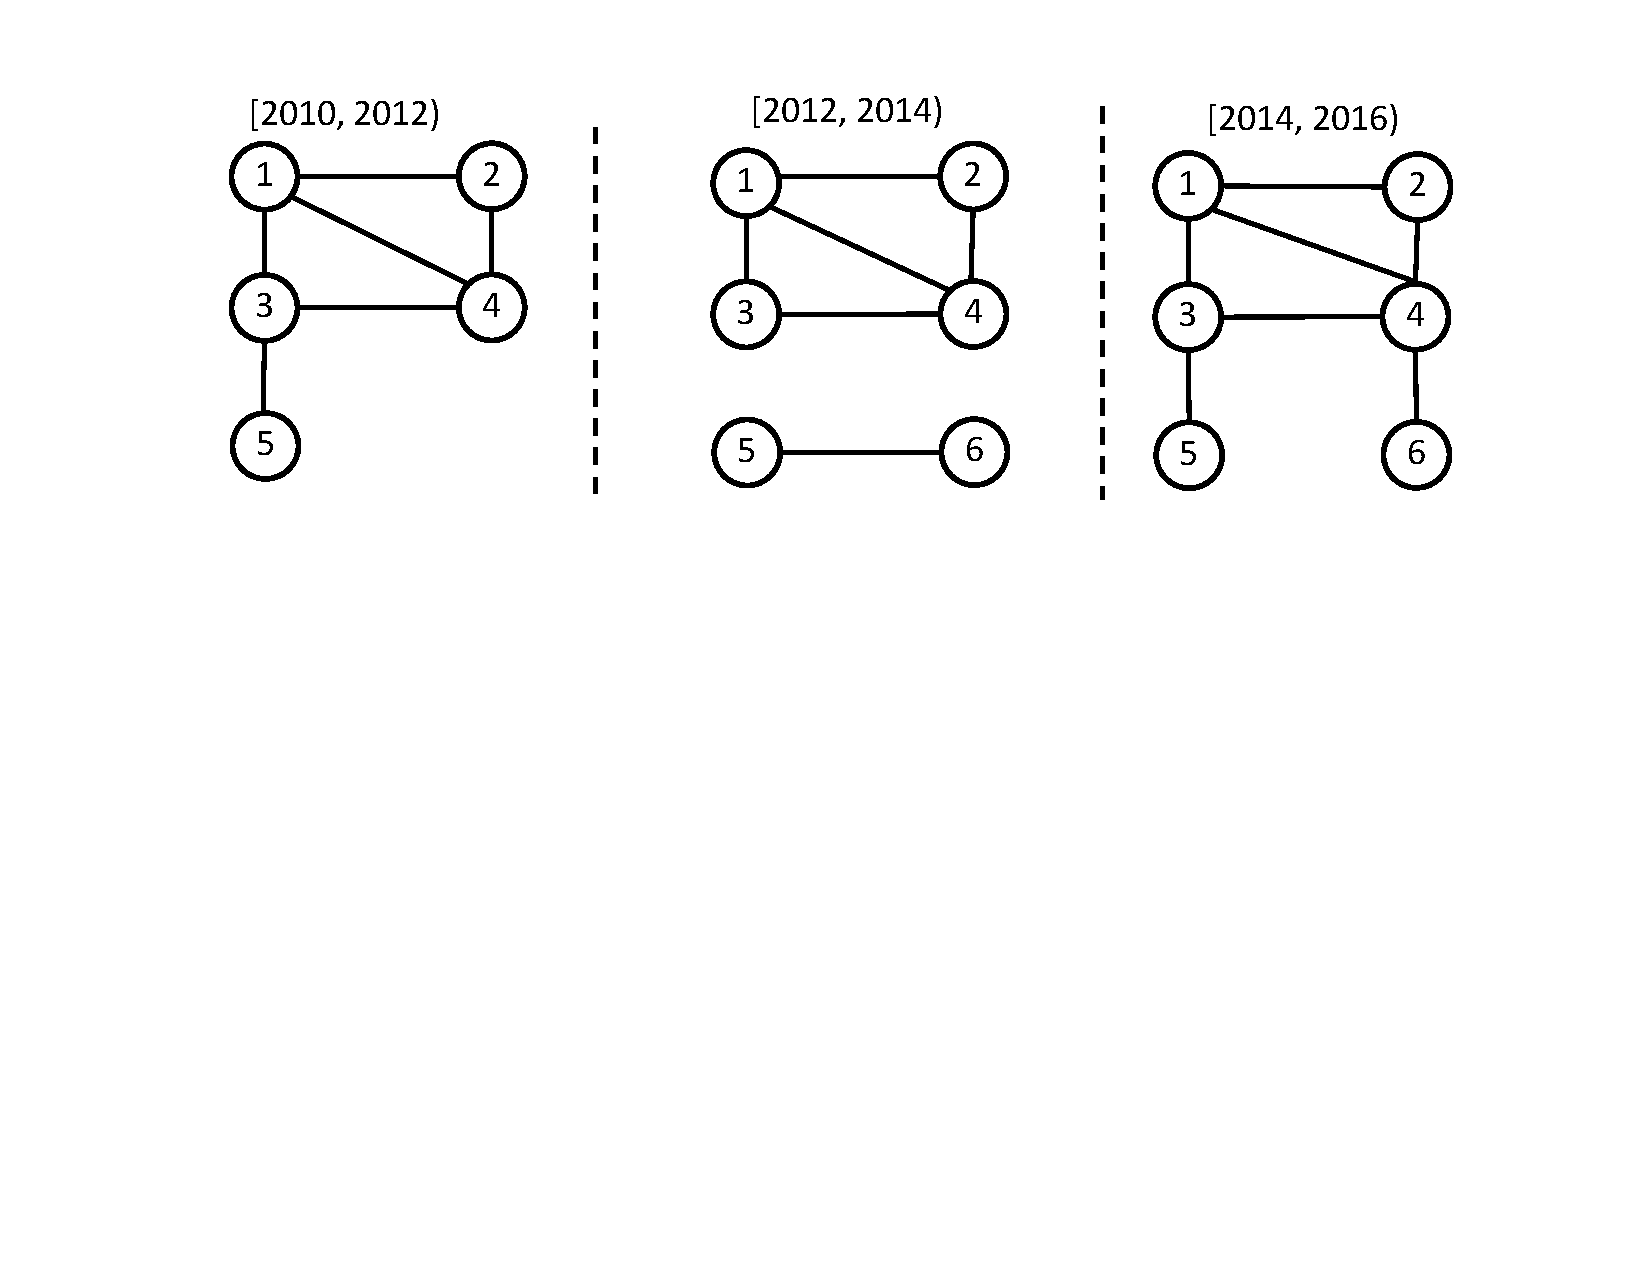
\includegraphics[width=2.5in]{figs/TGroupAny.pdf}
\vspace{-0.1in}
\caption{Result of query Q3 on T1.}
\label{fig:q3}
%\vspace{-0.1in}
\end{figure}

Consider next query $Q4$, and its result in
Figure~\ref{fig:tg_all_any}.

\begin{small}
\begin{verbatim}
Q4: TSelect All V [vid, any(name), max(salary)] ; 
            Any E [vid1, vid2, sum(cnt)] 
    From T1 
    TGroup by 2 years
\end{verbatim}
\end{small}

The main difference between $Q4$ and $Q3$ is the \insql{All} modifier
associated with vertices in the \insql{TSelect} clause of $Q4$,
meaning that $\gamma^{V}_{vid, any(name), max(salary)}(\bigcap_{G_i
  \in {\cal G}} V(G_i))$ (Definition~\ref{def:sgroup}) is used to
aggregate vertices of snapshots in each 2-year group.  \insql{Any E}
states that the edges in the result correspond to the union of the
edges connecting the vertices.\eat{  As our example illustrates,
\insql{Any} and \insql{All} modifiers are associated with vertices and
edges and are orthogonal, subject to the constraint that an edge can
only be present in a snapshot if both vertices it connects are
present.}

\begin{figure}
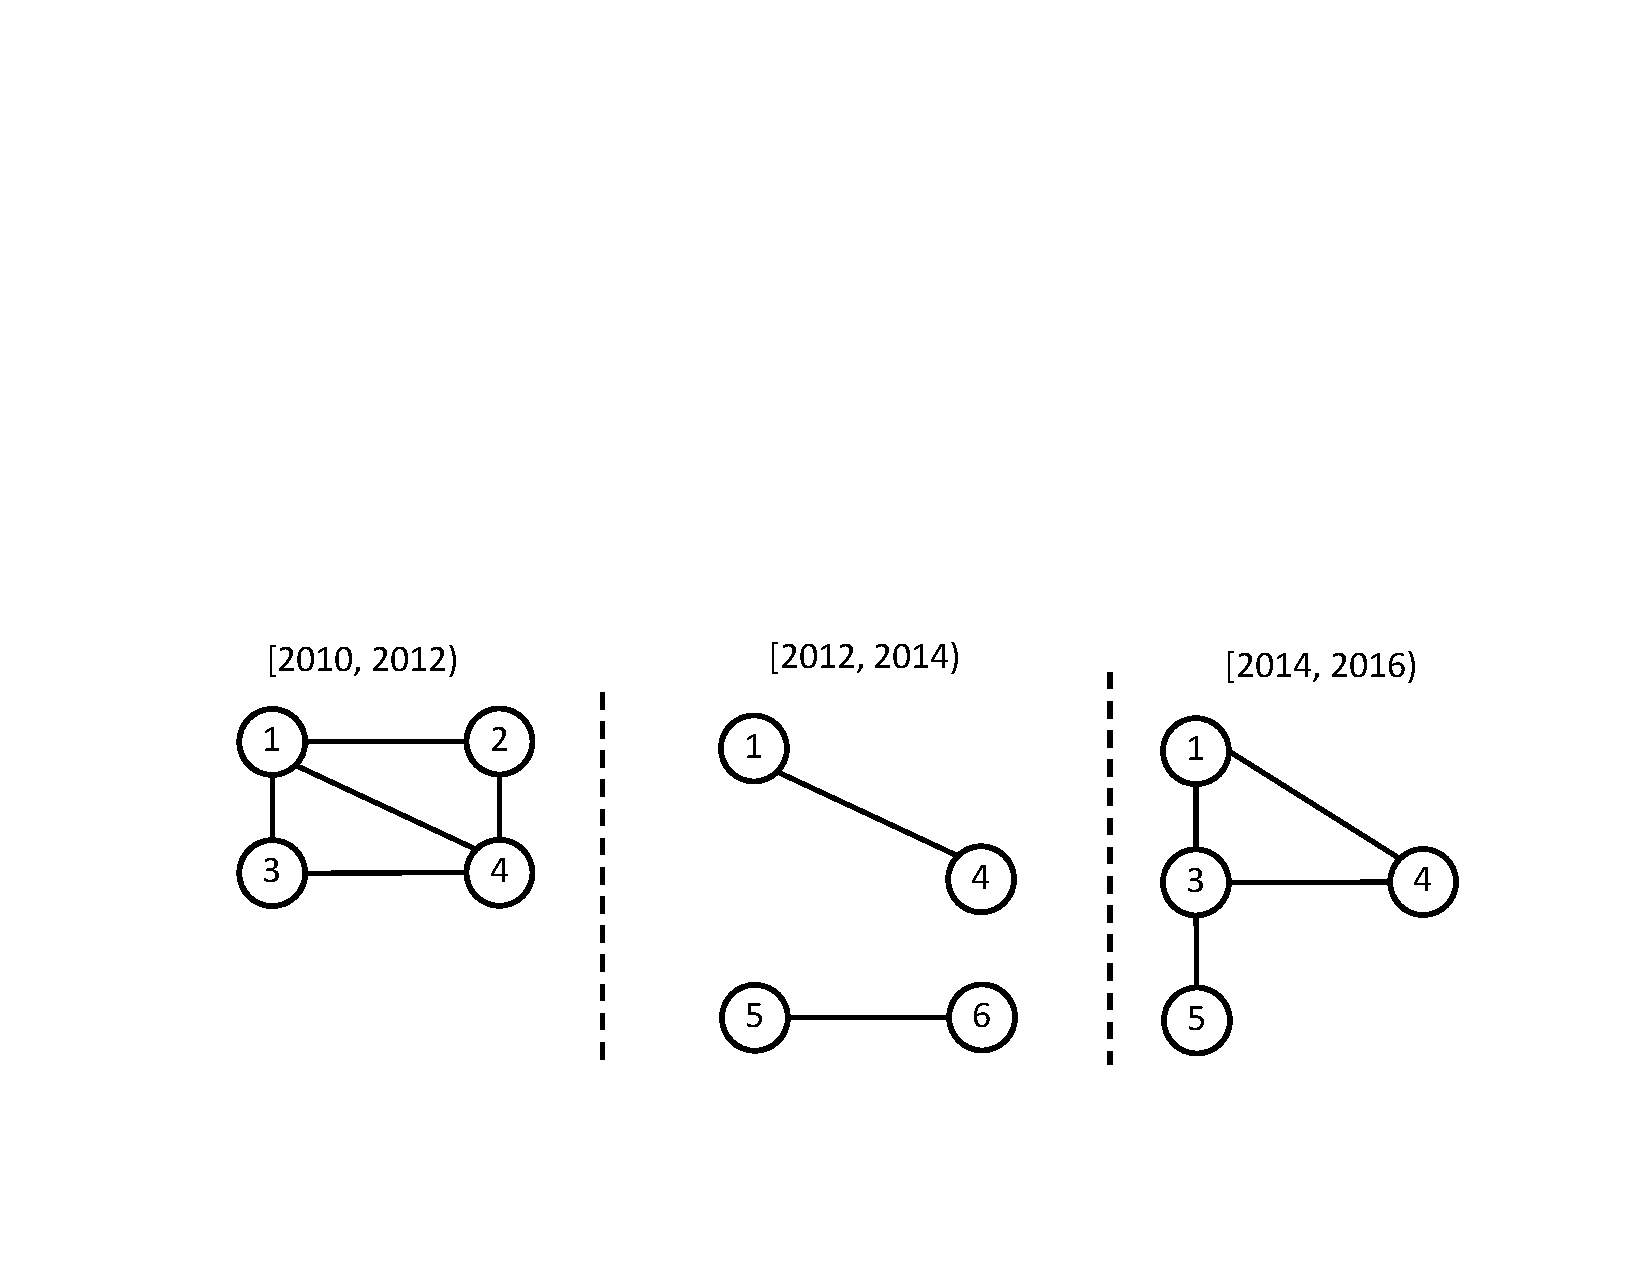
\includegraphics[width=2.5in]{figs/TGroupAllAny.pdf}
\caption{Result of query Q4 on T1.}
\label{fig:tg_all_any}
\vspace{-0.1in}
\end{figure}

$Q4$ illustrates another important feature of \ql, namely, aggregation
of values of non-key attributes of vertices and edges, which takes
place as part of structural aggregation.  We left available operations
unspecified in Definition~\ref{def:sgroup}, so as to keep structural
aggregation generic.
%
When used in scope of \insql{TGroup}, structural aggregation operates
over an ordered collection of snapshots.  \ql makes the following
aggregation operations available for ordered snapshot collections:
\insql{any}, \insql{first}, \insql{last}, \insql{min}, \insql{max},
\insql{sum}, \insql{count}, and \insql{list}.

To illustrate, consider vertex and edge relations in
Figure~\ref{fig:3ve}, which correspond to the first three snapshots of
\insql{T1}.  Vertex 1 is present in both $[2010, 2011)$ and $[2011,
    2012)$ in \insql{T1}, and so is present in the snapshot $[2010,
      2012)$ of the result of $Q4$.  Vertex 1 has \insql{name='Alice'}
      in both snapshots, but different values for \insql{salary}.
      Therefore, taking any value of \insql{name} and the maximum
      \insql{salary} may be appropriate.  Operations \insql{first} and
      \insql{last} return the value corresponding to the earliest
      (resp. latest) occurrence of an attribute, while \insql{list}
      returns a collection of all attribute values.

Returning to query $Q3$, when aggregation of attribute values is not
specified explicitly, \insql{any} is used as the default for non-key
attributes.  That is, the \insql{TSelect} clause of $Q3$ is short-hand
for \insql{TSelect Any V[vid, any(name), any(salary)] ;} 
\insql{Any E[vid1, vid2, any(cnt)]}.

\eat{
In the current version of \ql, temporal aggregation always groups
\insql{V} and \insql{E} by their respective key attributes, and values
of all other attributes are aggregated with one of the provided
operators (\insql{any} being the default).  In the future we will
support grouping by non-key attributes.  Further, we will define an
API to allow developers to specify custom aggregation operators.}

{\bf Temporal join.} We will now present two binary operators of \ql
that join together \tg relations, and will illustrate them using
\insql{T1} (Figure~\ref{fig:tg}) and \insql{T2}
(Figure~\ref{fig:tg_t2}).  Query $Q5$ computes temporal intersection
of \insql{T1} and \insql{T2}.  We require that \insql{T1} and
\insql{T2} be union-compatible, as per Definition~\ref{def:tuc}.  The
result of this query is in Figure~\ref{fig:q5}. 

\begin{small}
\begin{verbatim}
Q5:  TSelect   Any V; Any E
     From      T1 TAnd T2
\end{verbatim}
\end{small}

\begin{figure}
\centering
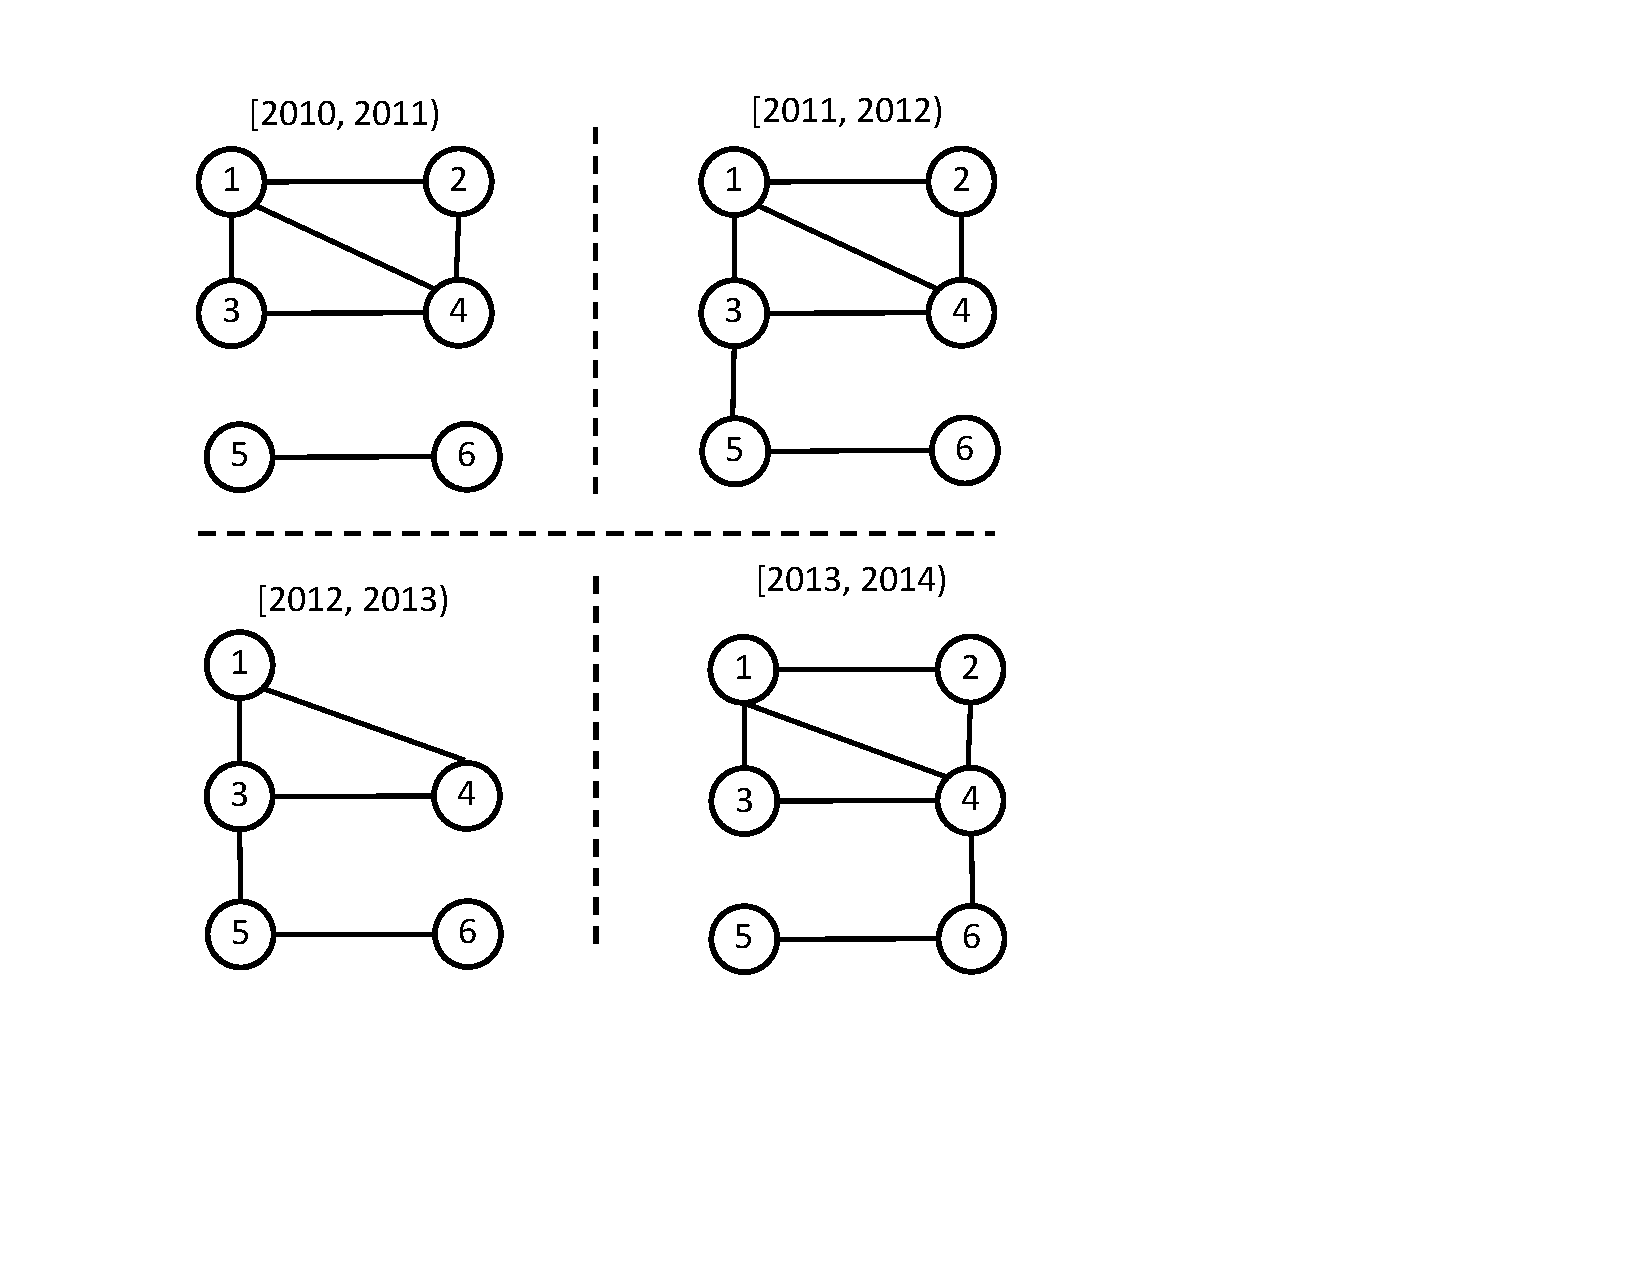
\includegraphics[width=2.8in]{figs/q5.pdf}
\caption{Result of query Q5.}
\vspace{-0.1in}
\label{fig:q5}
%\vspace{-0.1in}
\end{figure}

Temporal schema of the result is computed according to
Definition~\ref{def:tseqand}, and corresponds to a sequence with
$P.start = 2010$, $P.end=2014$ and $P.size=4$.  Note the use of
\insql{Any V} and \insql{Any E} in the \insql{TSelect} clause.  This
is another example of structural aggregation
(Definition~\ref{def:sgroup}), now as part of \insql{TAnd}.  The
modifiers \insql{Any} and \insql{All} have the same meaning here as
for \insql{TGroup}, specifying that, a vertex (resp. edge) will be
present in a snapshot in the result if it is present in at least one
corresponding snapshot of \insql{T1} or \insql{T2}.  

An important difference is that, for \insql{TAnd} and \insql{TOr},
structural aggregation operates on unordered collections of snapshots,
with at most two snapshots per group.  \ql makes the following
aggregation operations available for unordered snapshot collections:
\insql{any}, \insql{min}, \insql{max}, \insql{sum}, \insql{count}, and
\insql{list}.  Note that, unlike for \insql{TGroup}, \insql{first} and
\insql{last} are unavailable here, and that \insql{any} is still the
default.

\eat{
Also recall from our discussion of temporal aggregation that
\insql{TSelect Any V; Any E } is short-hand for \insql{TSelect Any V
  [vid, any(name), any(salary)]; Any E [vid1, vid2, any(cnt)]}.}


\eat{ Let us briefly revisit {\bf structural aggregation}, which is
  specified with \insql{Any} and \insql{All}, and has the same
  semantics in all \ql operators that map multiple input snapshots
  into one snapshot in the result. These operations are temporal
  aggregation, temporal union, and temporal intersection.  In all
  these operations, the use of \insql{Any} and \insql{All} for
  vertices and edges is orthogonal, subject to the constraint that an
  edge is only present in the result if both vertices connected by the
  edge are present.}

Consider next query $Q6$ that computes temporal union of \insql{T1}
and \insql{T2}.  The result of this query is shown in
Figure~\ref{fig:q6}.

\begin{small}
\begin{verbatim}
Q6:  TSelect   All V[vid, pagerank() as pr]; 
               Any E[vid1, vid2, sum(cnt)]
     From      T1 TOr T2
\end{verbatim}
\end{small}

\begin{figure}
\centering
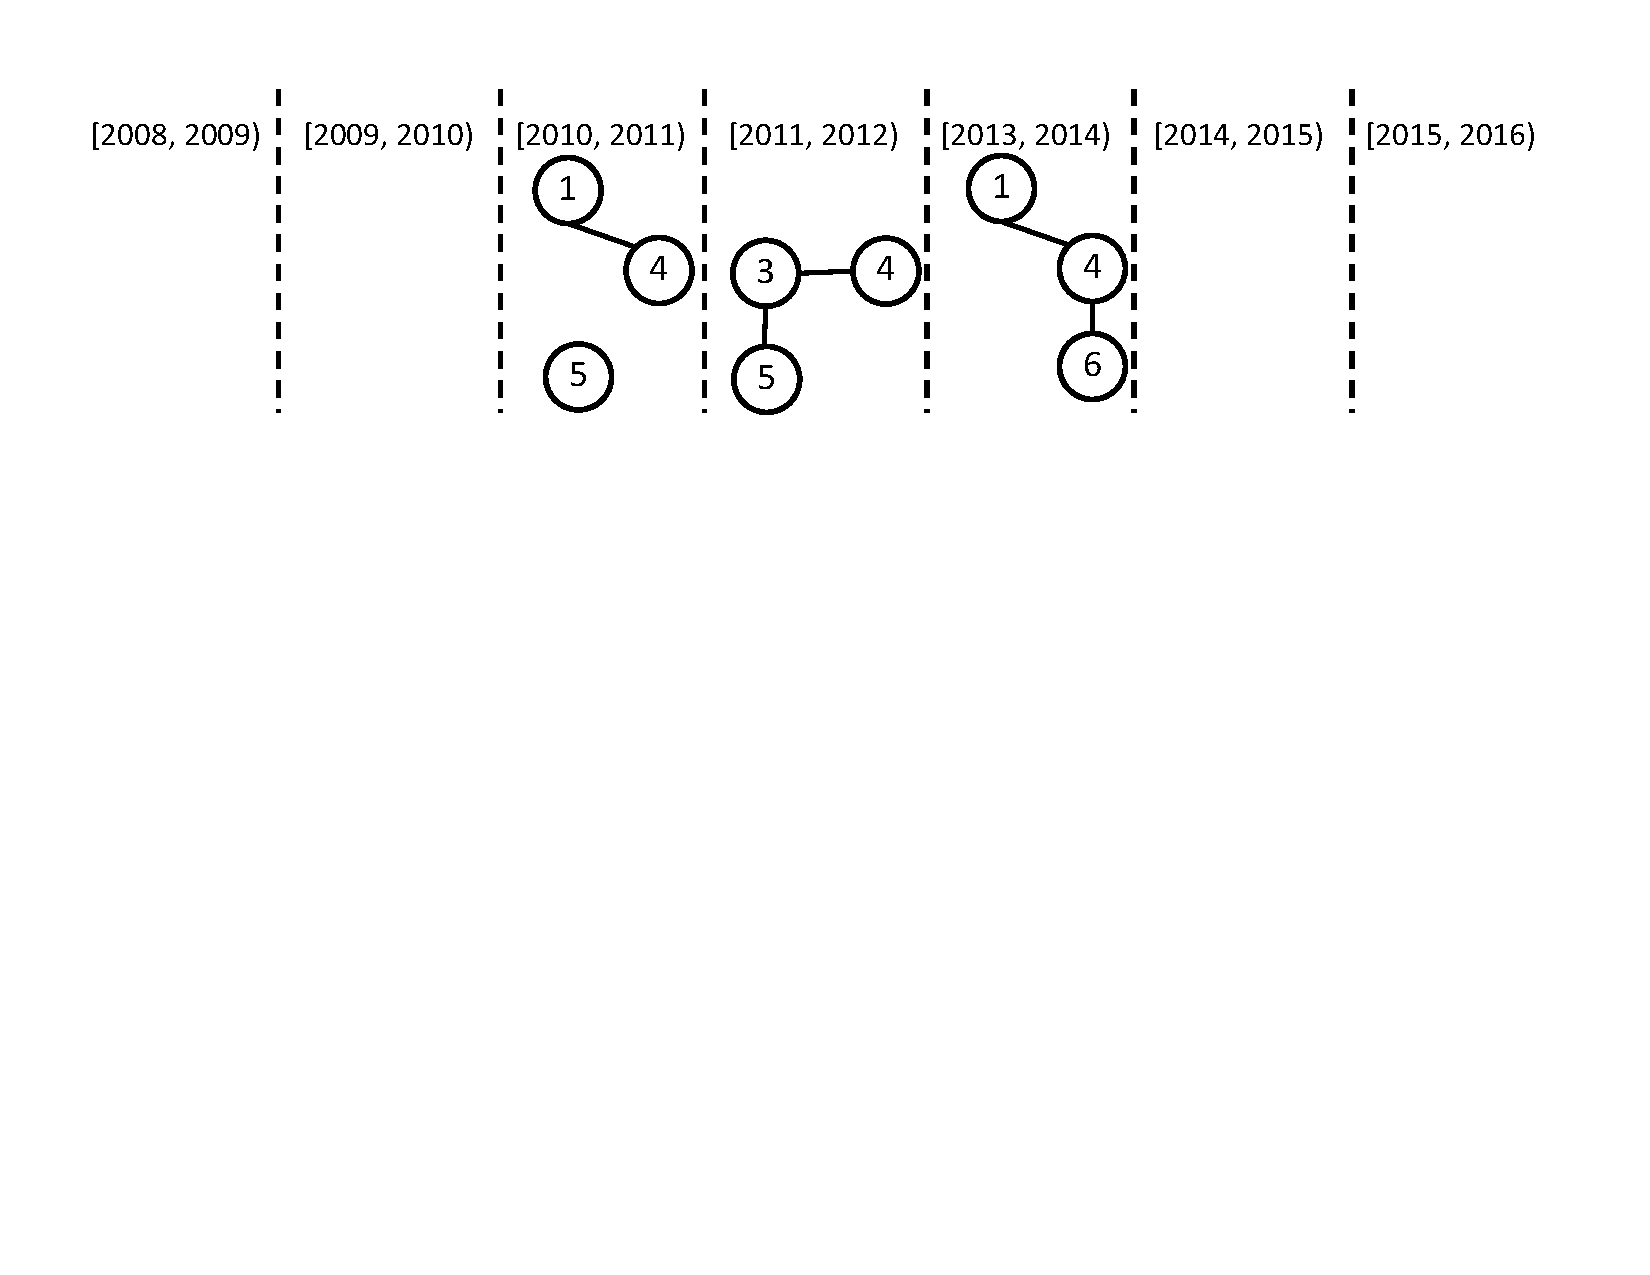
\includegraphics[width=3.3in]{figs/q6.pdf}
\vspace{-0.1in}
\caption{Result of query Q6.}
\label{fig:q6}
\vspace{-0.1in}
\end{figure}

Temporal schema of the result is computed according to
Definition~\ref{def:tseqor}, and corresponds to a sequence with
$P.start = 2008$, $P.end=2016$ and $P.size=8$.  Further, observe the
use of projection (non-key attributes of \insql{V} are not retained),
of an analytic function \insql{pagerank()}, and of the aggregation
operation \insql{sum} applied to the edge attribute \insql{cnt}.

\subsection{Complex queries}
\label{sec:example:complex}

{\bf Order of operators.} So far we illustrated individual operators
of \ql.  Now we will show how multiple operators can be combined in a
single query.  The logical order of evaluation of a \ql query without
nesting is as follows:

\begin{enumerate}
\item Temporal selection in the \insql{TWhere} clause;
\item Temporal join (\insql{TAnd} and \insql{TOr}) in the \insql{From}
  clause;
\item Temporal aggregation in the \insql{TGroup} clause;
\item Projection, computation of attribute aggregates and analytic
  functions.
\end{enumerate}

While the logical order of operations is predetermined, we will see in
Section~\ref{sec:sys:optimization} that some operators can be
reordered without affecting the result (but with potential differences
in performance), while others cannot.  

Consider $Q7$ below, with result shown in Figure~\ref{fig:q7}. $Q7$
first executes temporal selection on each \insql{T1} and \insql{T2}.
(Note that when temporal conditions in the \insql{TWhere} clause are
not qualified, they are applied to all \tgs in the \insql{From}
clause.)  Next, $Q7$ computes temporal intersection of \insql{T1} and
\insql{T2}, and then temporally aggregates the resulting \tg by 2
years.  Finally, \insql{pagerank()} is computed for each vertex in the
result.

\begin{small}
\begin{verbatim}
Q7:  TSelect Any V [vid, pagerank() as pr] ; 
             Any E [vid1, vid2] 
     From    T1 TAnd T2 
     TWhere  Start >= 2012 And End <= 2014 
     TGroup by 2 years
\end{verbatim}
\end{small}

\begin{figure}
\centering
\begin{minipage}{1.6in}
  \centering
  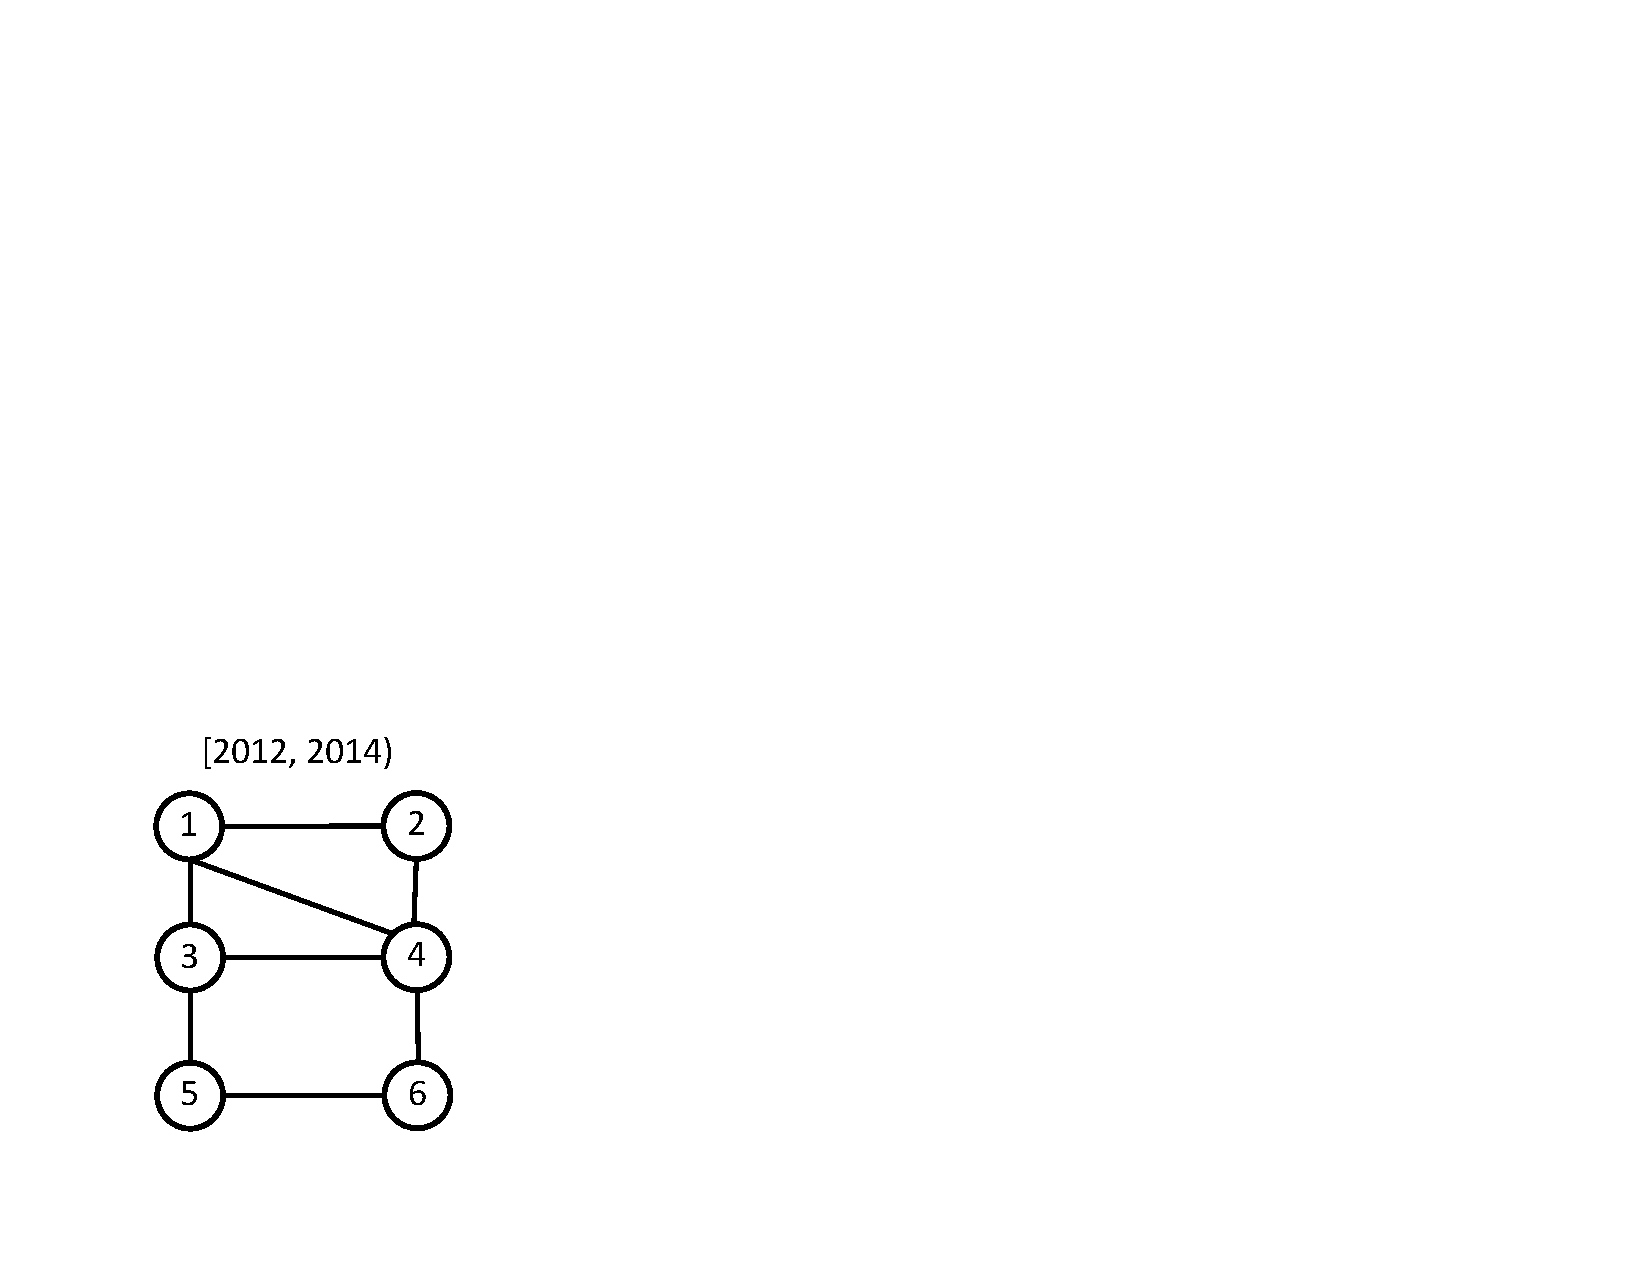
\includegraphics[width=0.8in]{figs/q7.pdf}
\vspace{-0.1in}
  \caption{Result of Q7.}{}
\vspace{-0.1in}
  \label{fig:q7}
\end{minipage}%
\begin{minipage}{1.6in}
  \centering
  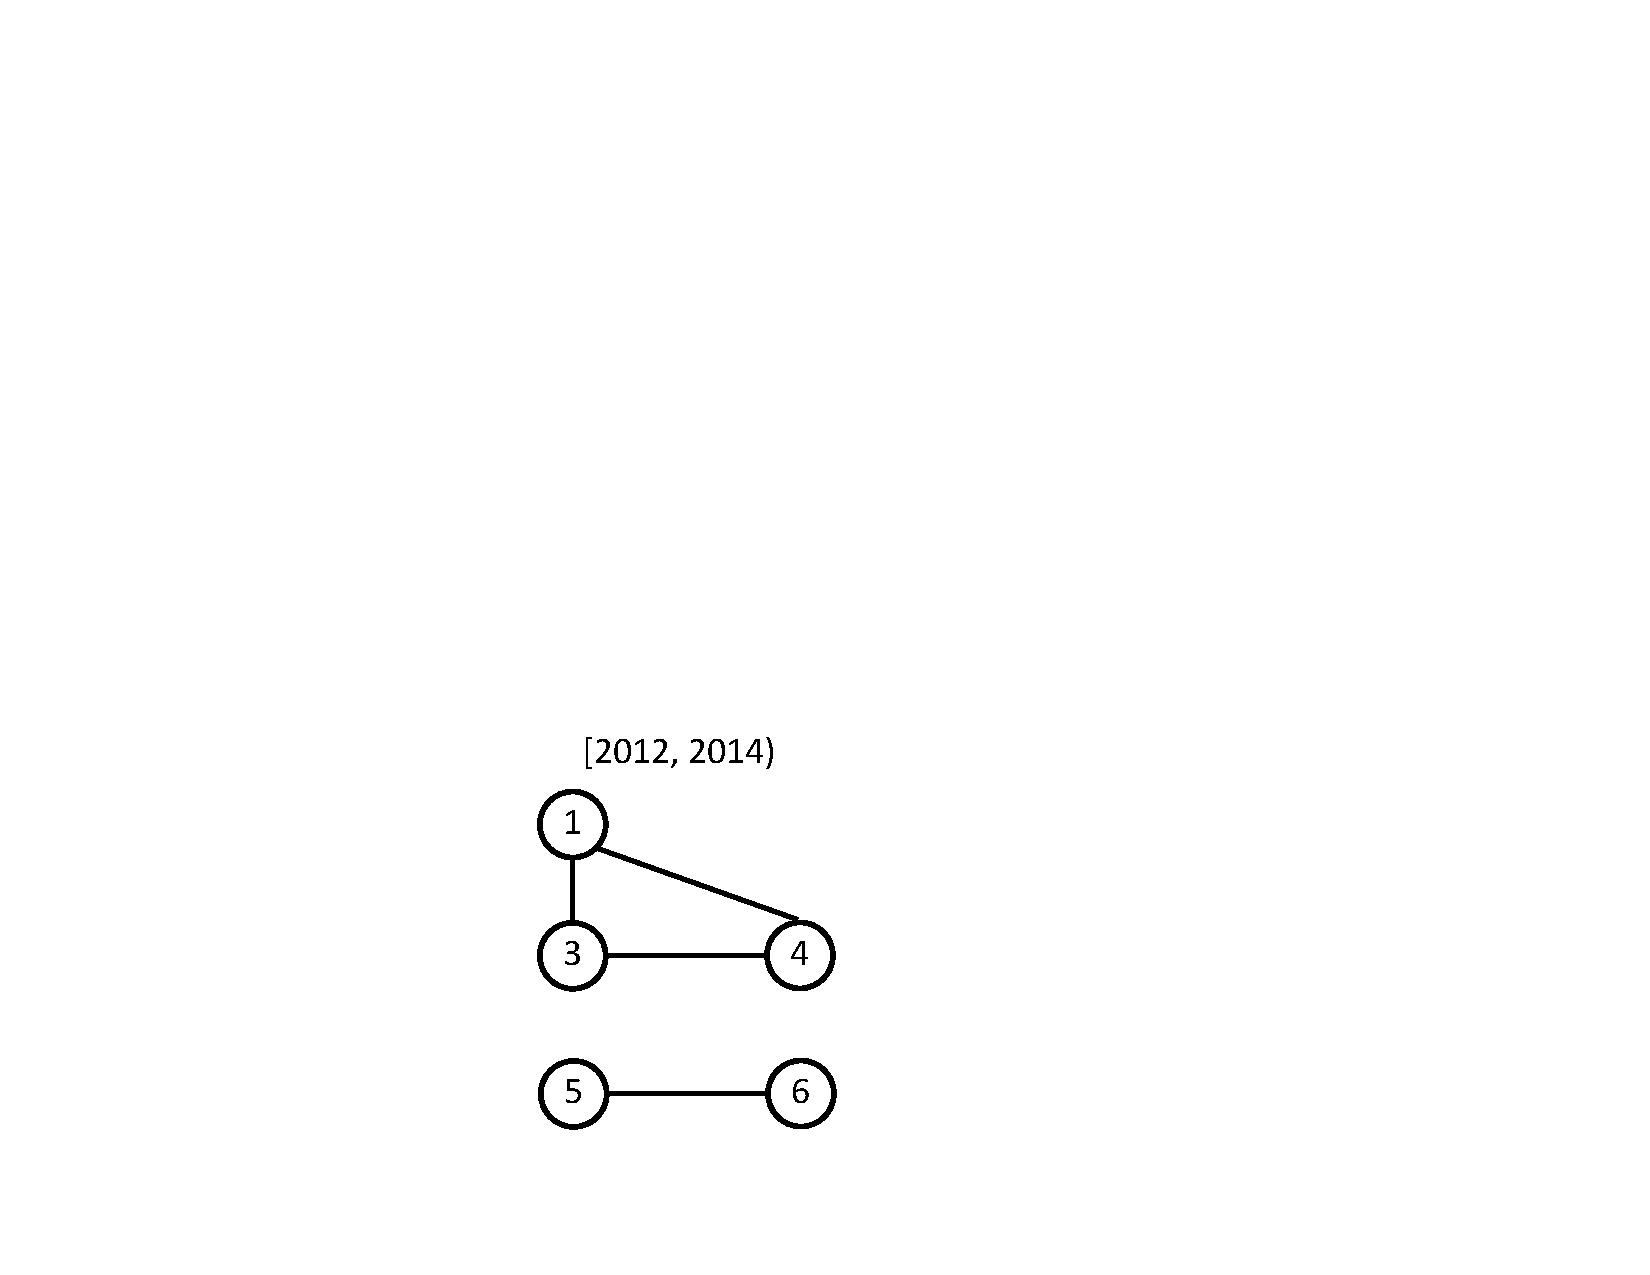
\includegraphics[width=0.8in]{figs/q8.pdf}
\vspace{-0.1in}
  \caption{Result of Q8.}{}
  \label{fig:q8}
\vspace{-0.1in}
\end{minipage}
\end{figure}

Observe that \insql{TAnd} and \insql{TGroup} use the same
specification in the \insql{TSelect} clause, that is, we cannot
decouple structural aggregation behavior of the two operations in a
query of this kind.

Consider next query $Q8$ that is similar to $Q7$, but uses nesting to
decouple structural aggregation of \insql{TSelect} from that of
\insql{TGroup}. The result of executing $Q8$ is shown in
Figure~\ref{fig:q8}.

\begin{small}
\begin{verbatim}
Q8:  TSelect   All V [vid, pagerank() as pr];
               All E [vid1, vid2]
     From      ( TSelect Any V [vid] ; 
                         Any E [vid1, vid2]
                 From    T1 TAnd T2
                 TWhere  Start >= 2012 
                 And     End <= 2014 )
     TGroup    by 2 years
\end{verbatim}
\end{small}

{\bf Trend analytics.} We argued in the introduction that it is
important to support analysis of trends in evolving graphs.  The \ql
query language makes this sophisticated analysis possible.  Query $Q9$
illustrates this; it invokes the snapshot analytic \insql{pagerank()}
on \insql{T1}, and then computes the trend in these values across all
snapshots.

\begin{small}
\begin{verbatim}
Q9:  TSelect Any V[vid, trend(pr) as tr, max(pr) as mx];
             Any E[vid1, vid2]  
     From    ( TSelect V[vid, pagerank() as pr];   
                       E[vid1, vid2]
               From    T1 )
     TGroup   by Size
\end{verbatim}
\end{small}

Consider the use of the {\em trend analytic} function
\insql{trend(pr)}, which aggregates the sequence of \insql{pagerank}
scores of each vertex.  In our implementation we use a common
definition of \insql{trend()}: compute the slope of the least squares
line using linear regression, making an adjustment when a vertex value
is missing.  While this is the only trend analytic we currently
support, we are working on an API that will allow developers to
implement custom trend analytics, taking attributes of both atomic and
complex type as input, and computing a value of either an atomic or a
complex type.

We invoke \insql{trend(pr)} alongside \insql{max(pr)} in $Q9$, to
highlight the difference between a trend analytic and value
aggregation.  Syntactically, the two look the same, but the difference
is that \insql{max(pr)} does not account for the temporal order of
values being aggregated, while \insql{trend(pr)} does.  Based on this
distinction, it is not meaningful to invoke a trend analytic when
structural aggregation is due solely to join (\insql{TAnd}) or 
(\insql{TOr}), but only as part of a query that does temporal
aggregation (\insql{TGroup}).

Finally, recall from our discussion of temporal aggregation that
\insql{TGroup by Size} produces a 1-snapshot \tg.  It is convenient,
although not required, to use this feature in a query such as $Q9$,
since a temporal trend may be computed over a window of any size.

\subsection{Loading data and inspecting results}
\label{sec:example:loadshow}

{\bf Loading filesystem data.  Views.}  Queries $Q1$ through $Q9$
refer to \tg variables in the \insql{From} clause.  The value of a \tg
variable is assigned by the \insql{Into} clause.  This value may be
loaded from the file system, as in query $Q10$, or it may correspond to
a view, as in query $Q11$.

\begin{small}
\begin{verbatim}
Q10:  TSelect V[vid:int, name:str, salary:int]; 
              E[vid1:int, vid2:int, cnt:int]
      From    path/to/directory
      Into    T3
\end{verbatim}
\end{small}

\begin{small}
\begin{verbatim}
Q11:  TSelect V; E
      From    T1
      Into    T4
      TWhere  Start >=  2010 
\end{verbatim}
\end{small}

Note that when data is loaded into a \tg variable from the file
system, as in $Q10$, the \insql{TSelect} clause must specify the
structural schema.  When a \tg variable takes on a value computed by a
query, its structural schema is determined by the query result.  In
$Q11$, the structural schema of the view \insql{T4} is the same as
that of \insql{T1}.

{\bf Inspecting results with SQL.}  Suppose that the result of $Q9$ is
assigned to \insql{T5}, with the structural schema
V(\underline{vid}:int, tr:float, mx:float) ; E(\underline{vid1}:int,
\underline{vid2}:int).  The SQL query below shows \insql{vid}
and \insql{tr} values of 20 vertices with the most significantly
increasing \insql{pagerank} trend.

\begin{small}
\begin{verbatim}
Q12:  Select   VF.vid, VF.tr  
      From     T5.toVerticesFlat() as VF
      Order by tr
      Limit    20
\end{verbatim}
\end{small}

The important part of \insql{Q12} is the use of
\insql{T5.toVerticesFlat()} in the \insql{From} clause.  This is a
multi-step operation provided by the \ql framework, which starts by
collecting all vertices in the union of snapshots of \insql{T5} into a
single nested vertex collection, and associating \underline{vid} with
a time-indexed map of vertex attributes.  Next, the nested collection
is flattened into \insql{VF} (\underline{vid}:int,
\underline{start}:date, \underline{end}:date, tr:float, mx:float).
\insql{VF} can be used in SQL queries.  The \ql framework also
provides an operation that returns a flattened collection of edges,
called \insql{toEdgesFlat()}.



